\section{Results}
\subsection{What each added mode changes}
Figure~\ref{fig:ablation} compares the hierarchy at four fixed points: weak finite-range coupling $(\eta,\delta_P,\xi)=(0.001,0.4,0.1)$; strong contact coupling $(10,1.2,0)$; a shape-dominated contact case $(0.372759\ldots,0.4,0)$; and a finite-range fixed-budget cancellation case $(0.263665\ldots,0.510345\ldots,0.1)$. Their mechanism labels concern the full solution, not a criterion for choosing the basis.

The first two columns expose why Hall sensitivity and ordinary conduction must be separated. M1 has no orthogonal active shape coordinate. Adding $u_2$ changes the active Hall readout strongly in the scalar example, reducing Hall error from 31.92\% to 0.681\%. Nevertheless its conductivity error remains 62.98\%, because passive current is frozen. In the contact shape example, M2 instead worsens Hall error from 2.063\% to 3.056\%. A physically meaningful added degree of freedom need not improve every functional monotonically. The variational property of a positive collision operator controls its energy norm, not the signed Hall functional.

M3 restores passive current. Both contact examples then agree with the full distribution within numerical precision, as the closure argument predicts. Thus passive current can transmit a Hall correction while having no Hall weight itself; its role is not confined to conductivity. The fourth mode contributes zero in this contact, massless limit.

Finite range changes the result. At the cancellation point, M1, M2 and M3 have Hall errors 4.146\%, 8.855\% and 16.869\%, respectively. M3 has already reduced conductivity error to 0.477\%. Adding passive valley polarization changes $H$ by $-0.966206$ and reduces Hall error to 0.01062\%; $Q_A$ error is 0.01152\%, while distribution error remains 1.894\%. The passive population thus supplies a distinct feedback pathway that ordinary conduction alone does not resolve. At the matched finite-range point $(1,1.2,0.05)$, M3 and M4 Hall errors are 7.095\% and 0.01207\%, confirming that the need for this mode is not confined to the near-cancellation example.

Conversely, at the weak point M1 already predicts $H$ to 0.0153\%, but misses conductivity by 74.56\% and the full distribution by 98.20\%. Four modes are not required there for a one-percent Hall prediction. They are required within this hierarchy for a common accurate description of the harder finite-range cases and of more than one observable. This conclusion concerns the tested ordered models, not a proof against every possible three-dimensional basis.

\begin{figure*}[!tp]\centering
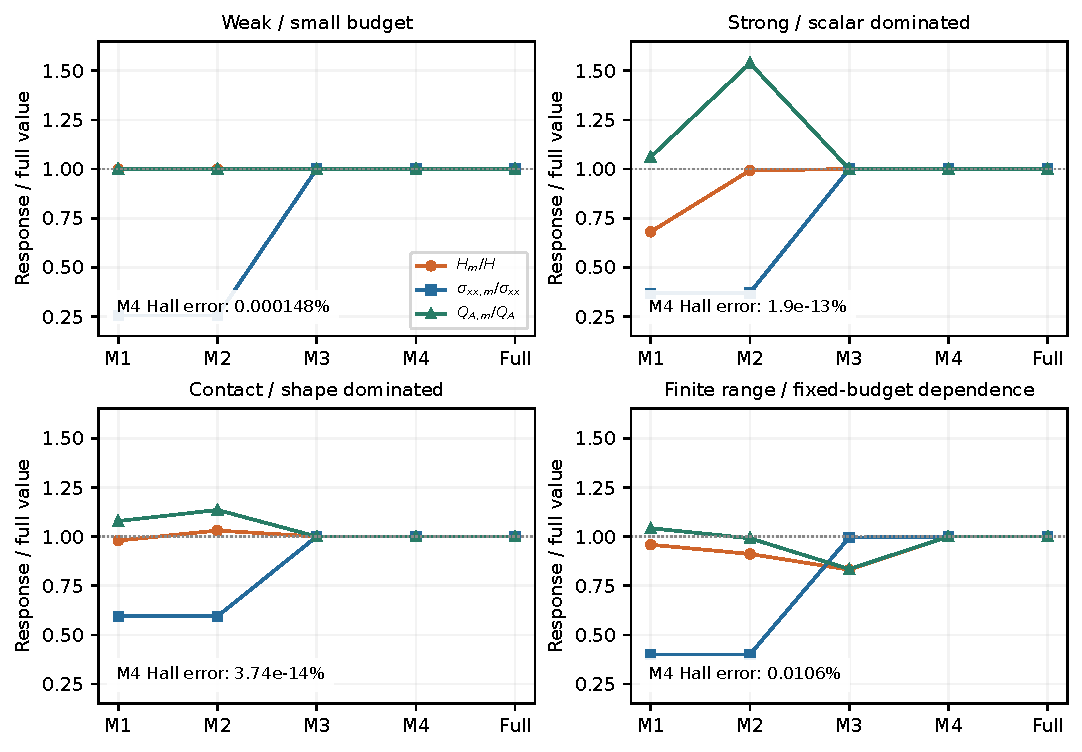
\includegraphics[width=\textwidth]{../figures/main/figure_2_ablation.pdf}
\caption{Physical mode ablation. Each panel compares normalized $H$, $\sigma_{xx}$ and $Q_A$ for M1--M4 and the full solution at the four points specified in Sec.~V.A. M1 is active reference current; M2 adds active valley distortion; M3 adds passive current; M4 adds passive valley population. All project the same full operator. Nonmonotonic Hall convergence is physical and is retained. Contact M3 is exact within numerical precision; finite-range M4 is approximate. Gaussian kernel, $m_P=0$, $N=256$ and common internal texture throughout.}\label{fig:ablation}
\end{figure*}

Across all 3510 positive-coupling principal-map points, M4's 95th-percentile and maximum relative Hall errors are 0.07267\% and 0.35751\%. Its maximum $\sigma_{xx}$ and $Q_A$ errors are 0.39543\% and 0.14630\%; its maximum weighted distribution error is larger, 4.58492\%. All 3510/3510 points meet one-percent accuracy for these three observables, whereas M3 meets that Hall criterion at only 1950/3510 points (55.56\%). Projection accuracy and sector-omission safety remain different questions: using M4 to estimate omission reproduces 3510/3510 decisions (100\%) at both 1\% and 5\%, and 3509/3510 (99.97\%) at 10\%. The one disagreement is false unsafe. These are sampled agreements, not certificates at unsampled boundaries.

\subsection{Closure, leakage and observable error}
Contact closure is analytic and numerical: the largest principal-map $\rho_{\rm rel}$ is $7.40\times10^{-15}$. On the positive-coupling two-kernel comparison, Gaussian finite-range residuals span $0.00648$--$0.03148$ at $\xi=0.05$ and $0.01512$--$0.06798$ at $\xi=0.10$. The corresponding Lorentzian intervals are $0.00536$--$0.02286$ and $0.01099$--$0.04736$. These are nonzero departures from an invariant space, not exact finite-range closure. Figure~\ref{fig:leakage} relates them to the projected response.

Leakage is informative but incomplete. Across the 2340 positive-coupling Gaussian finite-range points, its Spearman correlations with Hall, distribution and $Q_A$ errors are 0.606, 0.555 and 0.573. For Hall error the correlation changes from 0.774 at $\xi=0.05$ to 0.389 at $\xi=0.10$. Increasing leakage thus accompanies degradation in aggregate, but does not define a single error law. Equation~\eqref{eq:projectionerror} explains why: the omitted drive can compensate leakage forcing, and their residual must be weighted by the inverse collision operator and Hall readout.

The weak example makes the first effect explicit. The norms of $b_\perp$ and $R_{\rm inv}x_4$ are 0.00930086 and 0.00931814, but their difference has norm $8.07\times10^{-5}$. Most Frobenius leakage power lies above the median collision rate, and those leaked high-rate modes have small Hall overlap. Their combined response error is $-8.56\times10^{-6}$. This mechanism is consistent with the basis containing the exact uncoupled active response, despite a nonzero projection miss of the drive.

The difficult finite-range cases do not share a universal fast-mode explanation. At the matched Gaussian and Lorentzian points only 9.12\% and 8.18\% of leakage power lies above the median rate. At the cancellation point the exact spectral expansion
\begin{equation}
H-H_4=\sum_\nu\frac{(h^Tv_\nu)(v_\nu^Tr_b)}{\lambda_\nu}
\label{eq:spectralerror}
\end{equation}
has sum of absolute terms 0.301629 but signed sum $-0.000608821$. The full eigenmodes $v_\nu$ need not individually lie outside $U$; the leakage vector does. Degenerate subspaces are interpreted through summed residues. The Supplement displays leakage, drive and Hall weights.

Galerkin orthogonality gives another useful description. The exact Hall dual lies close to the retained space: $\norm{(I-P_U)z}/\norm z=0.00346$ at the cancellation point. Its orthogonal-residual bound in Eq.~\eqref{eq:dualbound} is 0.00394, compared with actual absolute error 0.000609. The simpler primal--dual residual bound is 0.0366 and is conservative. Accuracy therefore reflects a small omitted output sensitivity and signed modal compensation, not merely a small operator norm or uniformly fast leaked modes. These diagnostics do not establish robustness under arbitrary changes of bands or disorder.

\begin{figure*}[!tp]\centering
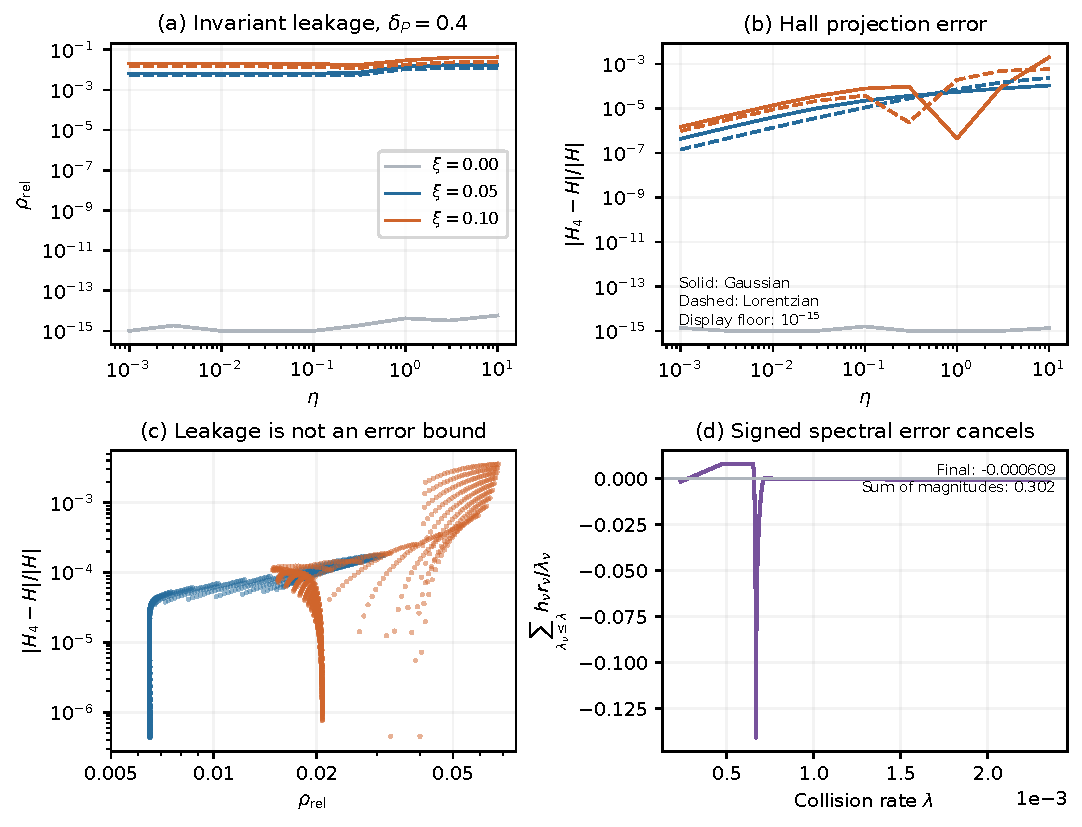
\includegraphics[width=\textwidth]{../figures/main/figure_3_leakage.pdf}
\caption{Invariant leakage and response accuracy. (a,b) Spectral residual and relative Hall error at $\delta_P=0.4$ on the fixed two-kernel grid; values below $10^{-15}$ are displayed at that floor. (c) All 2340 positive-coupling finite-range principal-map points. Each range contains 1170 points. Leakage is correlated with error but is not a bound. (d) Cumulative signed contributions to Eq.~\eqref{eq:spectralerror} at the fixed-budget cancellation point. The small final error results from compensated mode residues. All calculations use the fixed four-column basis and $N=256$.}\label{fig:leakage}
\end{figure*}

\subsection{Scalar, shape and signed compensation}
Define the component budget and cancellation diagnostics
\begin{align}
a&=|S|+|T|,\qquad B=a/|H_0|,\nonumber\\
f_{\rm sh}&=|T|/a,\qquad C=|S+T|/a.
\end{align}
Fractions are undefined at zero budget. We describe a nonzero correction as scalar or shape dominated when that component supplies at least 80\% of the absolute budget. These descriptive labels do not decide whether omission is safe.

For strong contact coupling, $S=2.23807$ and $T=0.0219153$: 99.03\% is scalar. The shape representative has $S=0.0472734$ and $T=0.190306$, or 80.10\% shape. The contact Hall overlaps are the same, $j_1=-0.0112813$, $j_2=-0.0643947$, so the active valley distortion has 5.708 times the readout per unit norm. The scalar case changes the reference amplitude by $-198.387$, with distortion amplitude $-0.340328$. In the shape case these are $-4.19040$ and $-2.95531$. Their residual shape forcings are comparable, but the shape case's stiffness is $0.00227649$, versus $0.0210367$ for the scalar case. A more weakly relaxed, Hall-sensitive distortion can therefore dominate a much smaller scalar change. The passive modes transmit the drive and feedback that set this competition.

At the finite-range cancellation point the reference-current amplitude increases while the active distortion has the opposite sign. Negative Hall overlaps then produce $S=-0.186970$ and $T=0.241183$. Figure~\ref{fig:mechanisms} compares these mechanisms with the weak, small-budget case. Cancellation between $S,T$ concerns the omission correction; cancellation among Eq.~\eqref{eq:spectralerror}'s residues concerns the projection error. They are distinct decompositions and should not be conflated.

\begin{figure*}[!tp]\centering
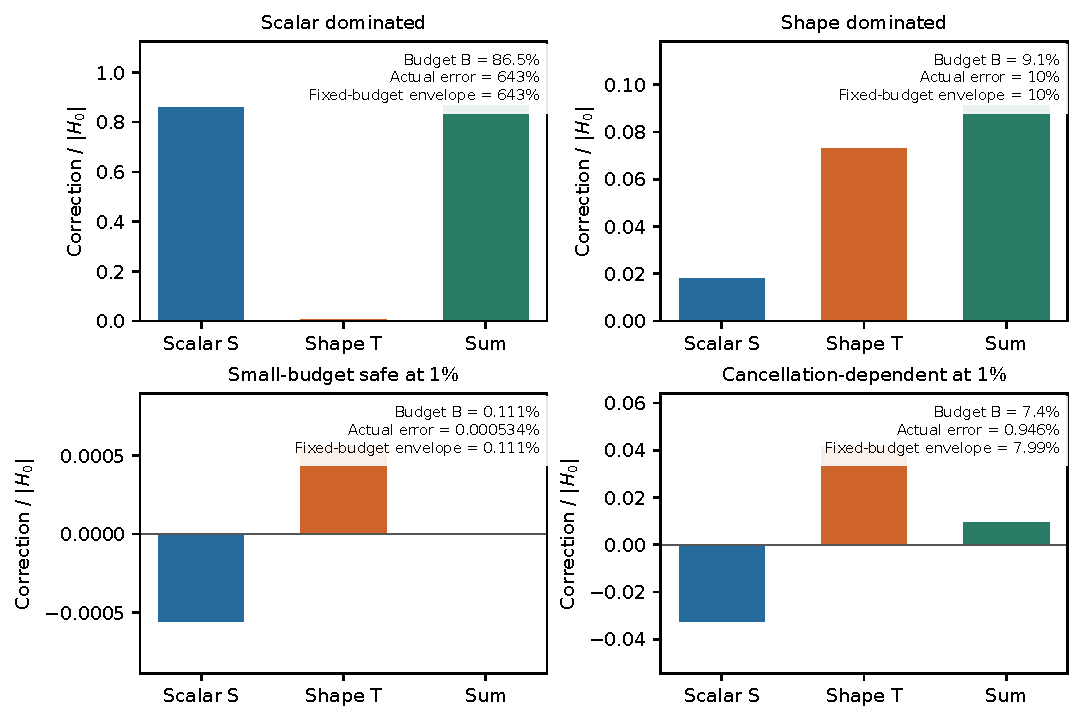
\includegraphics[width=\textwidth]{../figures/main/figure_4_scalar_shape.pdf}
\caption{Scalar and redistribution contributions to omission at the same four representative points as Fig.~\ref{fig:ablation}. Bars retain the signs of $S,T$ and their sum; annotations give the absolute budget, actual omission error and fixed-budget envelope. Strong cancellation at the weak point is irrelevant to a 1\% tolerance because its entire budget is small. The finite-range example is instead cancellation-dependent under the fixed-budget test at 1\%. Vertical scales differ to resolve each signed budget.}\label{fig:mechanisms}
\end{figure*}

\subsection{Tolerance decisions under the fixed-budget test}
Keep $|S|$ and $|T|$ fixed and ask whether removing their favorable signed cancellation could exceed the tolerance. For a possible net correction $D_c$ in $|D_c|\leq a$, the sharp interval/disk envelope is
\begin{equation}
e_{\rm fb}=\sup\frac{|D_c|}{|H_0+D_c|}
=\begin{cases}B/(1-B),&B<1,\\\infty,&B\geq1.\end{cases}\label{eq:envelope}
\end{equation}
For two real fixed magnitudes the discrete sign set is $\{\pm a,\pm(|S|-|T|)\}$. Its maximum agrees with this envelope for $B<1$, but need not diverge for $B\geq1$; both are saved. The test does not imply robustness to arbitrary physical perturbations, which can change the magnitudes themselves.

A well-conditioned point is robustly safe when $e_H\leq\epsilon$ and $e_{\rm fb}\leq\epsilon$. It is \emph{cancellation-dependent under the fixed-budget test} when $e_H\leq\epsilon<e_{\rm fb}$, and unsafe when $e_H>\epsilon$. Every dependent point here has opposing signs and $B<1$, so the discrete-sign and interval decisions coincide. Table~\ref{tab:decisions} reports the principal statistics using only $\eta>0$; zero-coupling controls are excluded.

\begin{table*}[t]\centering\small\setlength{\tabcolsep}{3pt}
\begin{tabular}{rrrrrr}\toprule
Tolerance & Safe / total (\%) & Robust / total (\%) & Dependent / total (\%) & Unsafe / total (\%) & Dependent / safe (\%)\\\midrule
1\% & 1410/3510 (40.17) & 839/3510 (23.90) & 571/3510 (16.27) & 2100/3510 (59.83) & 571/1410 (40.50)\\
5\% & 1942/3510 (55.33) & 1565/3510 (44.59) & 377/3510 (10.74) & 1568/3510 (44.67) & 377/1942 (19.41)\\
10\% & 2201/3510 (62.71) & 2065/3510 (58.83) & 136/3510 (3.87) & 1309/3510 (37.29) & 136/2201 (6.18)\\\bottomrule
\end{tabular}
\caption{Positive-coupling decisions on the principal Gaussian grid. Dependent means cancellation-dependent under the fixed-budget test. Undefined points are 0/3510 (0\%) at each tolerance. Safe includes both robust and dependent classes. Fractions describe this specified sampling grid, not a distribution of materials.}\label{tab:decisions}
\end{table*}

At the weak point $C=0.00479720$, yet $B\simeq0.001112$ and $e_{\rm fb}\simeq0.001113$. This is small-budget safe omission at 1\% and 0.5\%. At 0.1\% the same response is cancellation-dependent under the fixed-budget test, with actual error $5.3350\times10^{-6}$. Small $C$ alone cannot distinguish these decisions. The finite-range cancellation representative has actual error 0.9458\% but envelope about 7.99\%; it illustrates a decision-relevant compensation at 1\%. It is the maximum-envelope point among the grid's 1\%-safe dependent cases, a rule based on omission rather than ablation quality.

\begin{figure*}[!tp]\centering
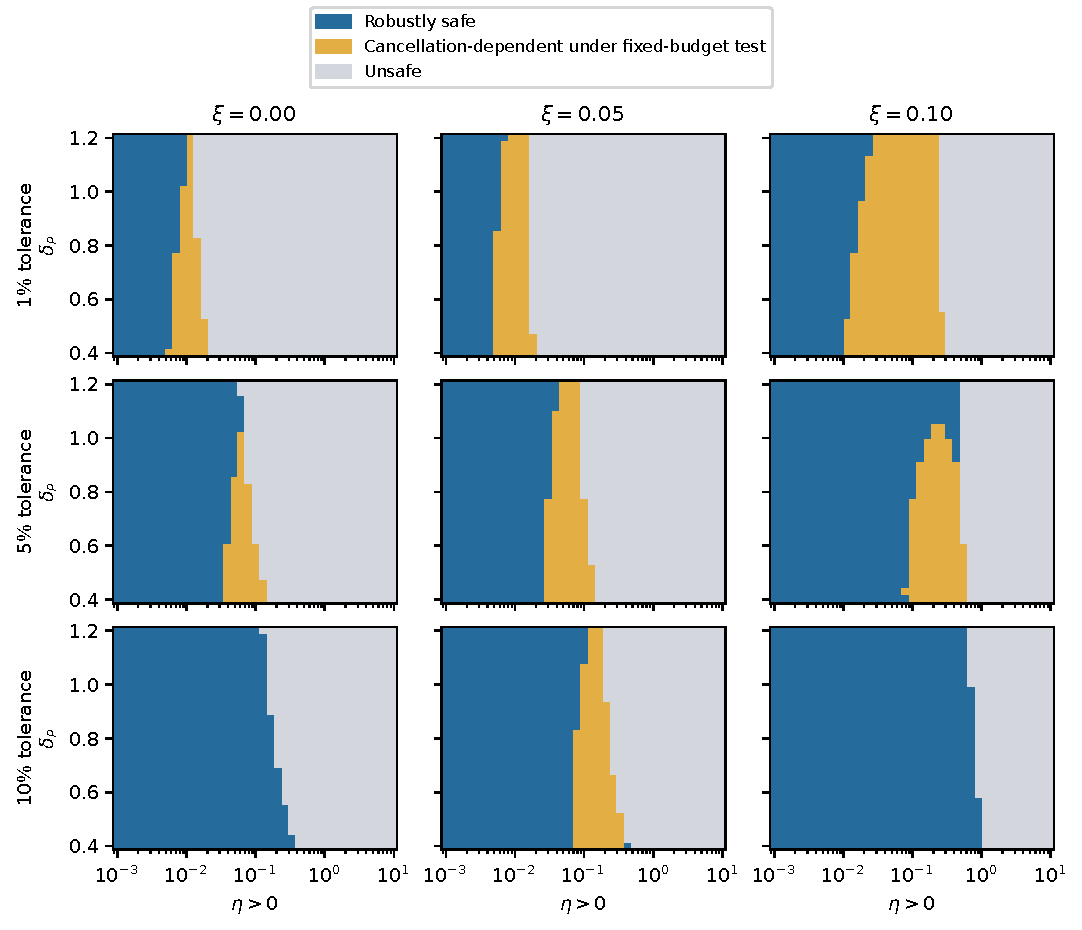
\includegraphics[width=0.96\textwidth]{../figures/main/figure_5_decision_map.pdf}
\caption{Observable-specific omission decisions for $\eta>0$. Rows use 1\%, 5\% and 10\% tolerances; columns use the three Gaussian disorder ranges. Blue is robustly safe, gold is cancellation-dependent under the fixed-budget test, and gray is unsafe. Each row contains the same 3510 positive-coupling points counted in Table~\ref{tab:decisions}; there are no undefined points. Boundaries are sampled, not analytically located. Fixed bands, common texture, $m_P=0$ and $N=256$ are used throughout.}\label{fig:decisions}
\end{figure*}

\subsection{Finite passive curvature}
When a passive mass is allowed, its direct readout must be restored. The correct separation is
\begin{align}
H_{\rm full}-H_0={}&H_P(0,m_P)+[H_A(\eta,m_P)-H_0]\nonumber\\
&+[H_P(\eta,m_P)-H_P(0,m_P)].\label{eq:masssplit}
\end{align}
These are respectively the direct passive baseline, active coupling and passive coupling corrections. For the untilted passive contour,
\begin{equation}
H_P=-\frac{m_Pv_P^2}{2\delta_P^3}(N_+-N_-),\quad
N_s=\sum_{i\in(P,s)}w_i\ell_i.\label{eq:polarization}
\end{equation}
The $N_s$ are driven displacements, not equilibrium densities. Finite-range intrapassive collisions can produce their difference even at $\eta=0$, which a constant-lifetime passive solution would miss.

At $(\delta_P,\xi,m_P)=(0.4,0.1,0.01)$, omission error is already 34.06\% without intersector coupling. At $\eta=0.001$ it is 35.61\%, and the three pieces of Eq.~\eqref{eq:masssplit} are $-2.987834$, $+3.69636\times10^{-5}$ and $-0.211288$. The direct baseline supplies 93.39\% of their absolute budget. The large mass-induced omission is predominantly direct passive readout, rather than active--passive kinetic reshaping. At fixed parameters $H_P/m_P$ approaches finite limits $-299.528$ and $-321.015$ at these two couplings. The mass controls and polarization figure are in the Supplement; no singular zero-mass limit or uniform mass tolerance is inferred.

\subsection{Observable dependence}
Ordinary conductivity makes sector omission a different question for an open-circuit conversion. The partial-channel factors are
\begin{equation}
K_E=-\frac{\chi(\omega)}{\sigma_{yy}(2\omega)},\qquad
K_J=-\frac{\chi(\omega)}{\sigma_{yy}(2\omega)\sigma_{xx}(\omega)^2}.
\end{equation}
The second denominator uses a complex square. Even at $\eta=0$, $m_P=0$, where $H=H_0$ exactly, the passive sector conducts. At $(\delta_P,\xi)=(0.8,0.05)$ the low-frequency ratios are $K_E/K_{E0}=0.26032$ and $K_J/K_{J0}=0.017392$. The derivation and frequency data are supporting results: these factors demonstrate observable dependence within the retained anomalous-velocity channel, not a complete device-voltage prediction.
